\documentclass[11pt,english,twocolumn]{article}

\usepackage{graphicx}
\usepackage{subfigure}

\title{Append-only Datastore}
\author{
	Mingyan Zhao \\
    myzh@stanford.edu
	\and
	Steven Tung\\
    steven.tung@stanford.edu
	\and
	Kevin Krakauer\\
    kevinkrakauer@gmail.com
}
\date{}

\begin{document}

\maketitle

% Calling our operation "put" is inherently confusing, I'm using "append".

\section*{Abstract}
We built an eventually consistent, append-only datastore focused on low
read/write latency and high availability. In the common case, clients interact
only with nearby nodes for extremely low latency. Data is always append to the 
store for a given key and the order is relatively kept.

The datastore is eventually consistent. Data is stored in memory for low latency
and in local disk for safety. Nodes can operate when disconnected from the
system, preserving availability in the face of total and long-term partitioning.
We believe this system will be useful in chat, social media and distributed logging
applications.

\vspace{-0.4cm}
\section{Introduction}
\vspace{-0.2cm}
As organizations increasingly move to the cloud, applications are designed from
the ground up with a distributed architecture (in some cases referred to as
\textit{microservices}). Despite numerous advantages, distributed
application design requires addressing latency and partitioning concerns that
monolithic applications do not have (or in the case of partitioning, are not
solvable).

Our \textit{append-only datastore} addresses latency and partitioning concerns
for append-only workloads. It is designed to run as a service distributed
globally across multiple data centers. By explicitly distinguishing between a
\textit{leader} node and \textit{follower} nodes, we gain several advantages
over other eventually consistent systems:
\begin{enumerate}
	\item Clients communicate only with their nearest follower for extremely
		low latency. \vspace{-0.3cm}
	\item Followers provide linearizability for client appends on a single
		key. That is, all clients writing to the same key of the same
		follower will see linearized writes.\vspace{-0.3cm}
	\item Data and its order is eventual consistency globally
\end{enumerate}
We also gain the advantages of some more traditionally eventually consistent
systems, such as great partition tolerance \cite{Dynamo}. Together, these
properties are highly desirable for many append-only applications. Consider the
following:

\begin{itemize}
	\item \textbf{Distributed logging} - Consider a monitoring service using the append-only datastore records logs in real time. The service writes and retrieves logs with extremely low latency from the nearby data center. Also it is provided an eventually consistent log that has the data from all of the deployments.
	\item \textbf{Chat Application} - Consider a chatroom
		occupied by a team in North American and a team in Asia. Each
		team member sees their local peers' messages immediately and in
		exactly the order that they are sent.
\end{itemize}

\section{Related Work}
Amazon's Dynamo \cite{Dynamo} supports always-writable semantics, high partition
tolerance, and laser-focuses on low-latency operation. Unlike our system, Dynamo
is a key-value store. It also exposes a great deal of complexity to developers,
who have to tailor their use of Dynamo such that conflicts are resolvable and
must manually implement conflict resolution in clients. Our system does not
allow for conflicts. Google's GFS \cite{GFS} is also optimized for append-heavy workloads and uses a
single master for simplicity and intelligent coordination. It supports random
writes as well. However, it is explicitly optimized for non-latency-sensitive
applications, and a single read can require multiple hops (the GFS master and
chunkserver). LinkedIn's Kafka \cite{Kafka} provides eventual delivery of large
quantities of data, but running under a publish/subscribe
mechanism.

\vspace{-0.4cm}
\section{Design}
Nodes in the append-only datastore are classified in a simple hierarchy as seen
in Figure \ref{Architecture}. A single \textit{leader} directs multiple
\textit{followers}. Clients connect to and communicate with a nearby follower,
likely running in the same data center, to minimize latency. Our design tolerates
arbitrary partitions between nodes and ensures an eventually consistent view of
data.
%\vspace{-0.4cm}
% Architecture
\begin{figure}[t]
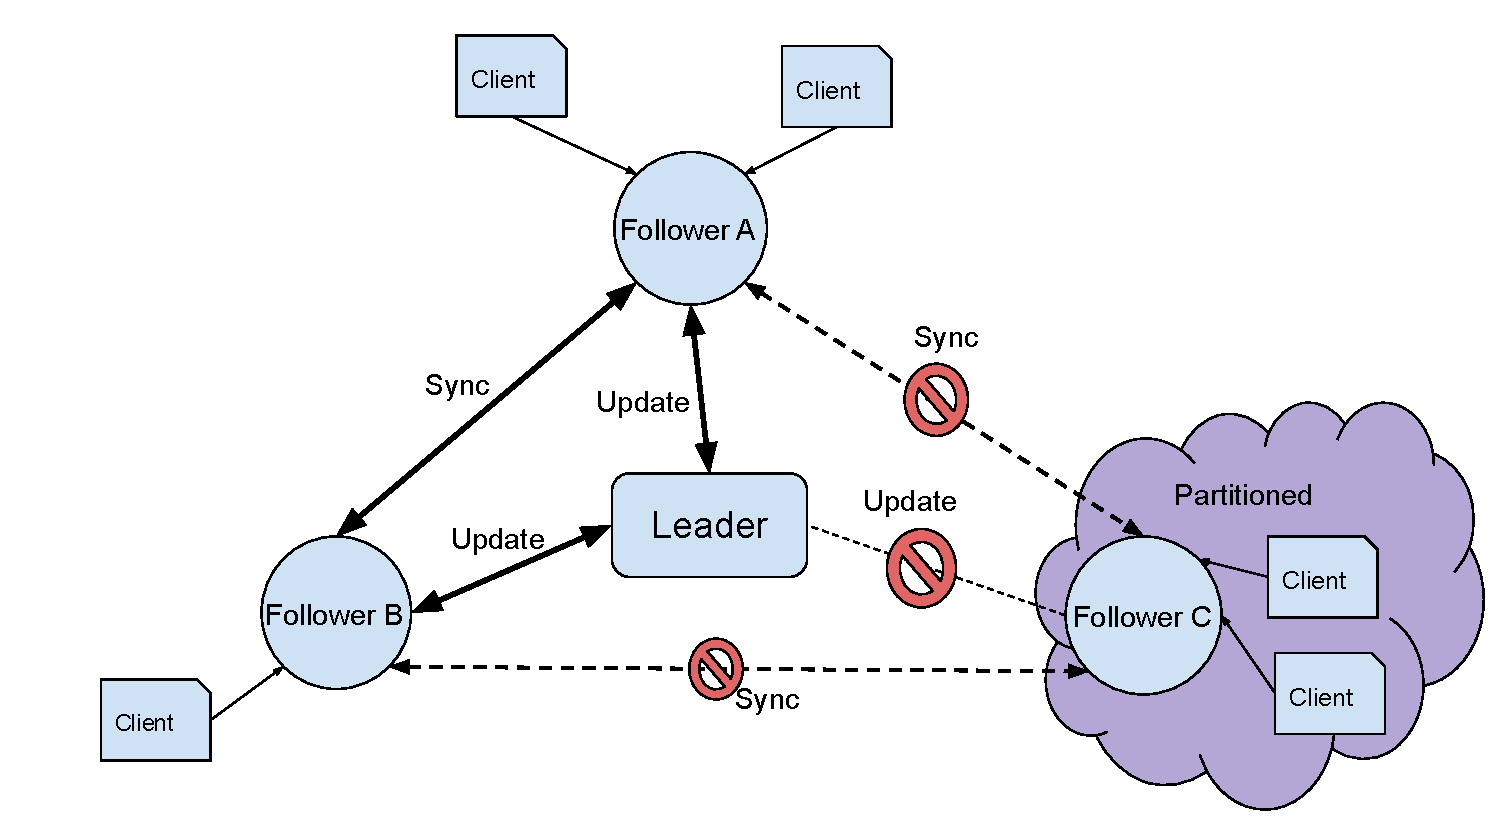
\includegraphics[width=8cm]{figure/SystemStructure.pdf}
\caption{Architecture}
\label{Architecture}
\end{figure}
Clients are exposed the following API by followers:
\begin{itemize}
	\item \texttt{append(key, data)} - Appends \texttt{data} to the existing
		data for \texttt{key}. Guarantees that \texttt{data} is safe if data is written in local disk.
	\item \texttt{get(key)} - Gets the data for \texttt{key}, represented as a
		list of values. Data written by the same client is guaranteed to be in the same order, but new data may appear later.
\end{itemize}

\subsection{Leader}
% TODO: Explain what happens when this is partitioned. Look at gfs paper.
The leader is responsible for globally ordering writes for each key. Like GFS's
master \cite{GFS}, it only stores metadata rather than the value itself.
This decreases network usage.  Also, the
burden on disks is lighter per update, increasing writes per second and the
average lifetime of each disk. The simplicity of a single master
simplifies our implementation and the rest of our design, which increases
the overall stability of the system. 

\subsubsection{Index number}
The Leader maintains the latest index number for all keys. The index numbers are globally unique and monotonically increasing. Once generated, it will be mapped to a list of value on the requesting follower. If another follower needs that value, it simply needs the index number to fetch the data. The index numbers are protected by mutex lock to avoid conflicting update. 

 \vspace{-0.4cm}
\subsubsection{Update}
Upon receiving an \texttt{Update} request, the \texttt{Leader} advance the index number by one and update the follower information to the incoming one. Each key entry is locked before updating to avoid concurrent write issue.

The \texttt{Leader} decides if the requesting follower needs to sync up with other followers. If a mapping exists from key $k$ to index $i$, an \texttt{Update} carrying the same index $i$ does not need an Sync (the $i$ still increments by 1). This may happen when 1)  a key created on the \texttt{Leader} for the first time, or 2) the requesting follower is the same as the recorded follower for the key.

An \texttt{Update} to $i' < i$ indicates that the sender is not holding the latest data. In this case the leader signals it to sync with the follower in its records that originated the append at index $i$. This may happen when two followers are appending data to the same key alternatively. A common case is shown in Figure \ref{CommonUpdate}.

% update procedure figure
\begin{figure}[h]
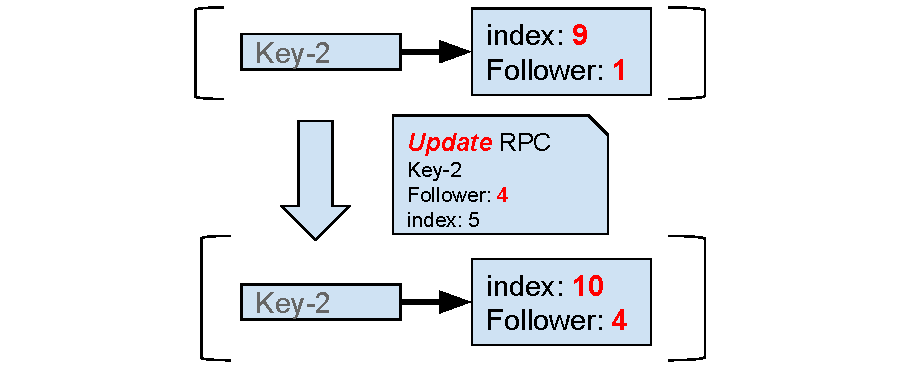
\includegraphics[width=8cm]{figure/update.pdf}
\caption{Update procedure}
\label{CommonUpdate}
\end{figure}

\vspace{-0.3cm}
\subsubsection{Broadcasting index numbers}
The broadcasting of the \texttt{Leader} ensures the eventual consistency of the system. The new appended value gets replicated and synced immediately between the requesting followers and in-record follower, but all of the other followers would not know it until the \texttt{Leader} broadcasting the latest index number. 

Depending on the workload and use cases, we provide different ways of broadcasting. One is triggered per-request, which is expected to provide lower consistency latency but may only be used in a lower QPS scenario, since the broadcasting may cause a great amount of communication between the followers. The other one is triggered periodically, which is expected to be used in most cases. The \texttt{Leader} only broadcasts the updated keys and their index numbers in a short period of time.

\subsubsection{Leader Fault Tolerance}
Because the leader writes all updates to disk, it tolerates crashes and reboots.
For greater fault tolerance, it should write to multiple disks or a remote disk
as well.

The system continues to function when the leader is partitioned, but followers
and thus clients do not receive updates from other followers. As long as the
partition is eventually healed, the system will propagate information correctly
and self-heal. If for some reason there is a permanent partition, it must be
manually worked around by changing the cluster configuration (i.e. the set of
nodes in the system).

\subsection{Follower}
% Explain what happens when this is partitioned.
% Explain read-your-own-writes consistency.
% Be sure to discuss any synchronization that happens here, as the follower is
% responsible for synchronizing its the writes to it.
The follower is our most critical component. Its responsibilities include:

\begin{itemize}
	\item Handing \texttt{append} and \texttt{get} requests. \vspace{-0.4cm}
	\item Managing data. \vspace{-0.4cm}
	\item Updating the leader about appended data. \vspace{-0.4cm}
	\item Syncing with other followers to communicate updates and orderings.
\end{itemize}

\subsubsection{Data structure}
Followers replicate the entire datastore in memory to minimize
reading and writing latency. The data structure is described in Figure \ref{DataStructure}.

% data structure figure
\begin{figure}[h]
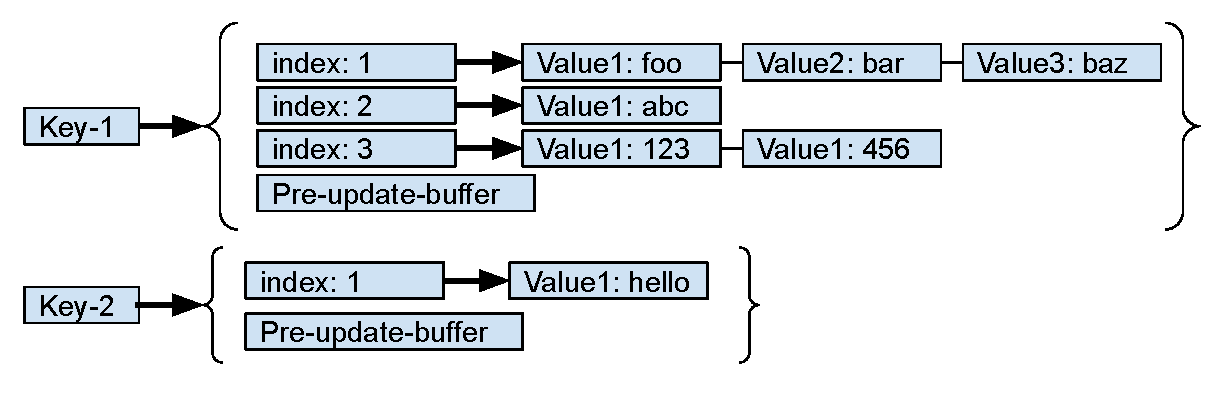
\includegraphics[width=8cm]{figure/DataStructure.pdf}
\caption{Data procedure on Follower}
\label{DataStructure}
\end{figure}

\subsubsection{Client Interfaces}
\textbf{Append(key, data):} Upon reviving \texttt{Append} request, the follower write the data to memory first and then write to a local disk for data safety. It returns immediately after the data is written to local disk. For increased fault
tolerance, the append should be written to multiple disks locally or to a remote
disk as well. Note that throughout this section when we refer to updating local
storage, the in-memory store is also updated immediately after data is written
to disk.

The follower always appends the data to the pre-update-buffer firstly, then issues an \texttt{Update} if the pre-update-buffer is not empty. If it receives an \texttt{Update} response with a index number, it creates an new index entry and moves all of the data from pre-update-buffer to the new entry. 

\noindent \textbf{Get(key):} When clients issue a \texttt{Get} requests, they are served from the in-memory datastore. It guarantees that the data written by the local clients are up-to-date but it is not globally consistent. The follower builds up a list with all of the data from each index as well as everything from the pre-update-buffer.

\subsubsection{Synchronization}
Followers use the \texttt{Sync} request to get data they missed. This ensures the eventual consistency of the system. \texttt{Sync} requests also signal what data the sender has to the recipient, enabling the recipient to create new index entries in its local datastore. The \texttt{Sync} request is issued when a follower receives an \texttt{Update} response from the \texttt{Leader} indicating it needs synchronization. 

Since a follower may missing multiple indices of data, a \texttt{Sync} request may carries a list of indices that it is asking for. However the recipient may also missing some of the indices if there is a large amount of \texttt{Sync} requests on the flight everywhere. To mitigate this, the \texttt{Sync} response only reply with indices and the data the recipient already has, so that the issuer could accept what are returned and do another \texttt{Sync} asking for what is left. Eventually, each follower will synchronize with  other ones and achieves the globally consistency.

Combining with the \texttt{Update} requests, the Figure \ref{UpdateAndSync} demonstrates a message flow of synchronization in common case.

% UpdateAndSync figure
\begin{figure}[h]
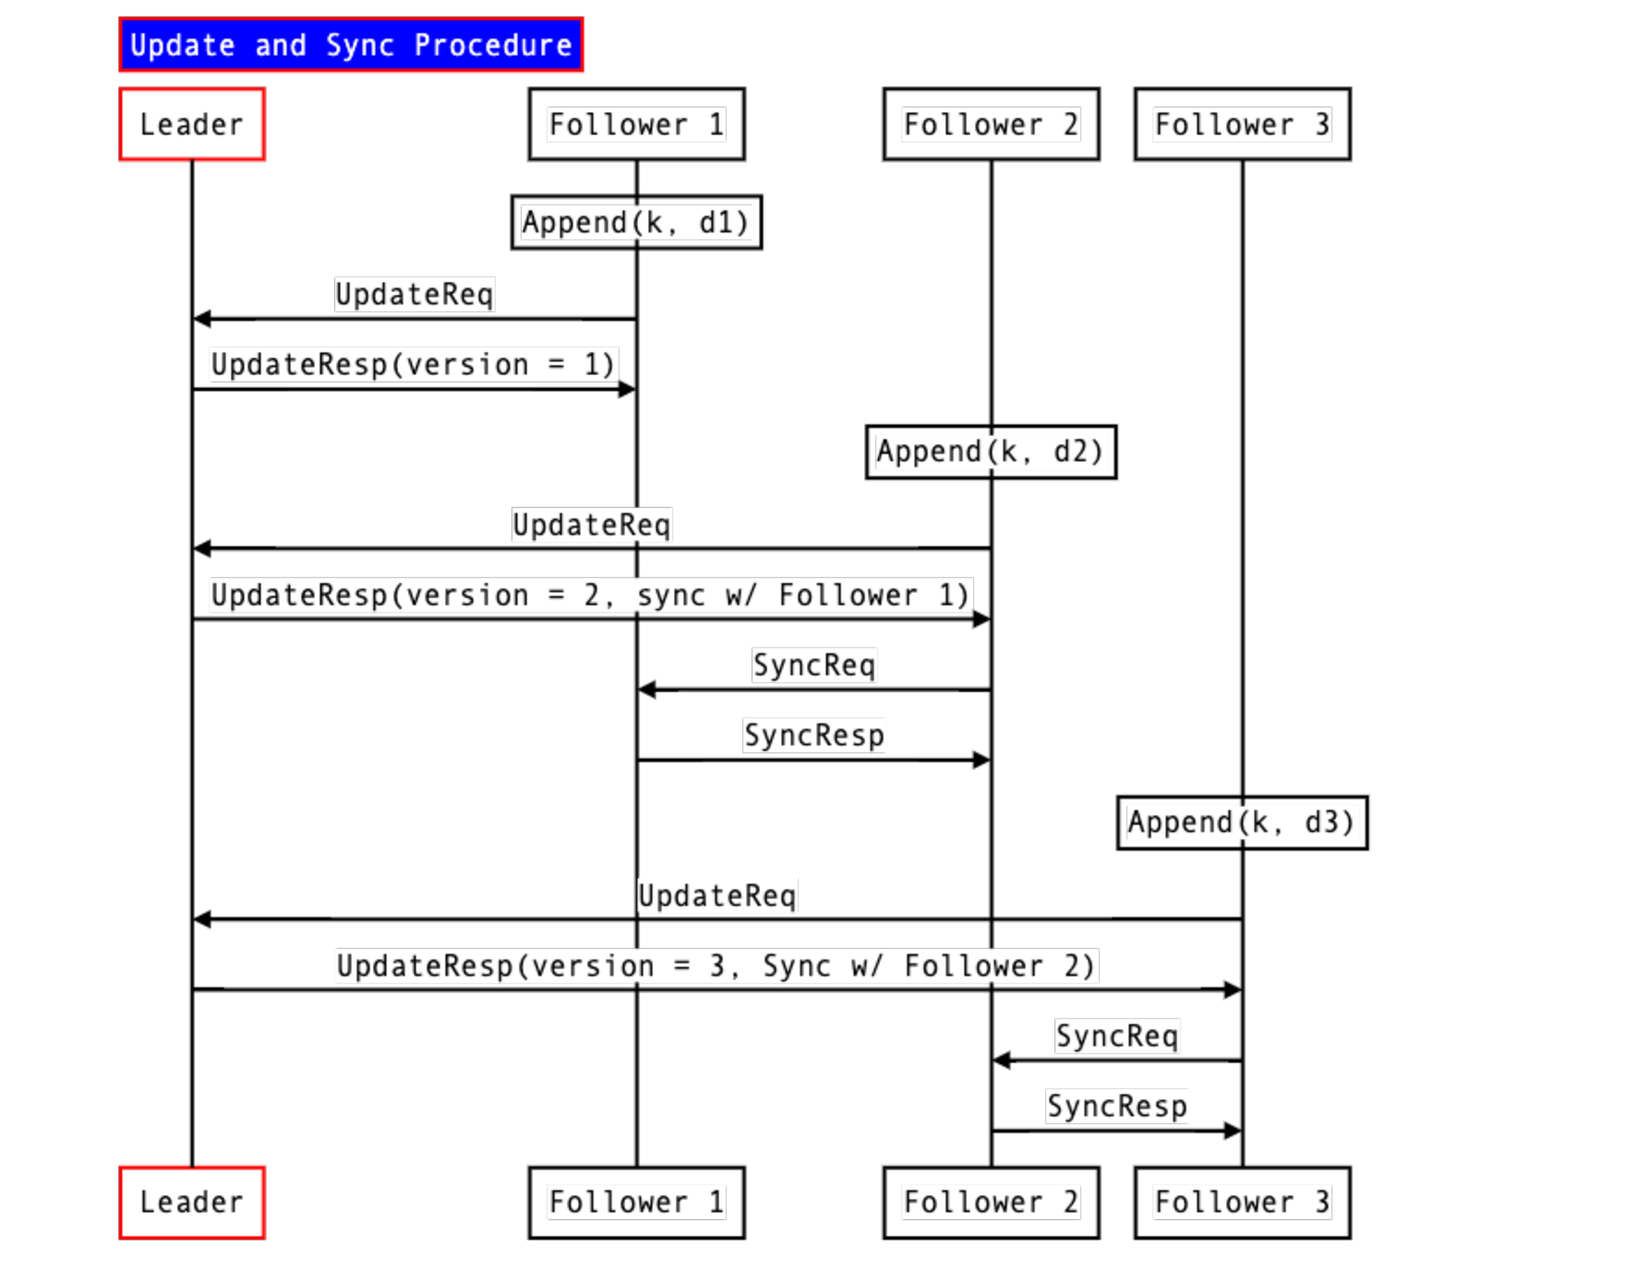
\includegraphics[width=8cm]{figure/UpdateAndSync.pdf}
\caption{Update and Sync message flow}
\label{UpdateAndSync}
\end{figure}

\subsubsection{Follower Fault Tolerance}
Both \texttt{Update} and \texttt{Sync} requests are retried in case of network
failure. If a follower reboots during a \texttt{update}, it can inspect the disk
at boot and see that it has appended data locally that has not been confirmed by
the leader. If a follower reboots during a \texttt{sync}, it will have stale
data until a \texttt{get} or \texttt{append} causes it to update. This keeps the
system simple while retaining its consistency properties.

\vspace{-0.4cm}
\section{Evaluation}
The system is written in Go and can be run manually or distributed and
run with Docker. Nodes communicate via gRPC. 

We ran tests with a cluster of Google Compute Engine virtual
machines. Google Cloud platform provides internal IP address communication between VM instances, which means the request among servers would not need to go through public network so that the speed would be much faster. We deployed our system in the following locations.
\begin{itemize}
    \vspace{-0.4cm}
	\item One leader in Iowa, Central USA.
	\vspace{-0.4cm}
	\item One follower and one client in each of the following five locations
\vspace{-0.3cm}
    \begin{itemize}
    \item Iowa, central USA.
\vspace{-0.3cm}
	\item Los Angeles, west USA.
\vspace{-0.3cm}
	\item South Carolina, east USA.
\vspace{-0.3cm}
    \item London, west Europe.
\vspace{-0.3cm}
    \item Tokyo, northeast Asia.
\vspace{-0.3cm}
    \end{itemize}
\end{itemize}

In the performance test, each client in the performance test sends 120,000 \texttt{Append} against 10 keys randomly, so that in total there would be 600,000 values in the datastore globally. After all of the \texttt{Appends} are done, each client then retrieves the data by issuing \texttt{Get} for all of the 10 keys every 0.5 second periodically.

 \vspace{-0.5cm}
\subsection{Append Request Performance}
We measures the \texttt{Append} request latency firstly, see Table \ref{AppendLatency}. The result shows that the speed of \texttt{Append} is extremely fast, which is about 7.5 millisecond in average. And the 600,000 requests can be done in a little less than 1 second, so that the performance test can be considered as showing a QPS performance of our system.

\begin{table}[h]
\small
\centering 
\begin{tabular}{ |p{1.6cm}|p{1cm}|p{0.8cm}|p{0.8cm}|p{1cm}|p{0.8cm}|  }
\hline
Location & S. C. & Tokyo & Iowa & London & L.A. \\
 \hline
 1 Req   & 8.06 & 7.91 & 8.23 & 7.82 & 7.94\\
\hline
600k Req & 967.62 & 948.72 & 988.00 & 938.75 & 952.92\\
 \hline
\end{tabular}
\caption{Append request latency in millisecond(S.C. for South Carolina, L.A. for Los Angeles)}
\label{AppendLatency}
\end{table}

 \vspace{-0.5cm}
\subsection{Eventual consistency}
One critical result is the eventual consistency, since this is what we trade off for the low latency read and write. The result is shown in Figure \ref{ConsistencyDelay}. We can see after 0.5 second, all of the Followers have already started syncing with each other and received some of the data from each other. The start point is different since the clients were started not at exactly the same time. After 2.0 seconds, we can see that the Follower deployed in South Carolina finished synchronization and received all of the 600,000 values. After 3.5 seconds, all of the follower were holding all of the data and the system reached the eventual consistency.

% Consistency delay figure
\begin{figure}[h]
	\subfigure[Eventual Consistency Delay]{\label{fig:c}
		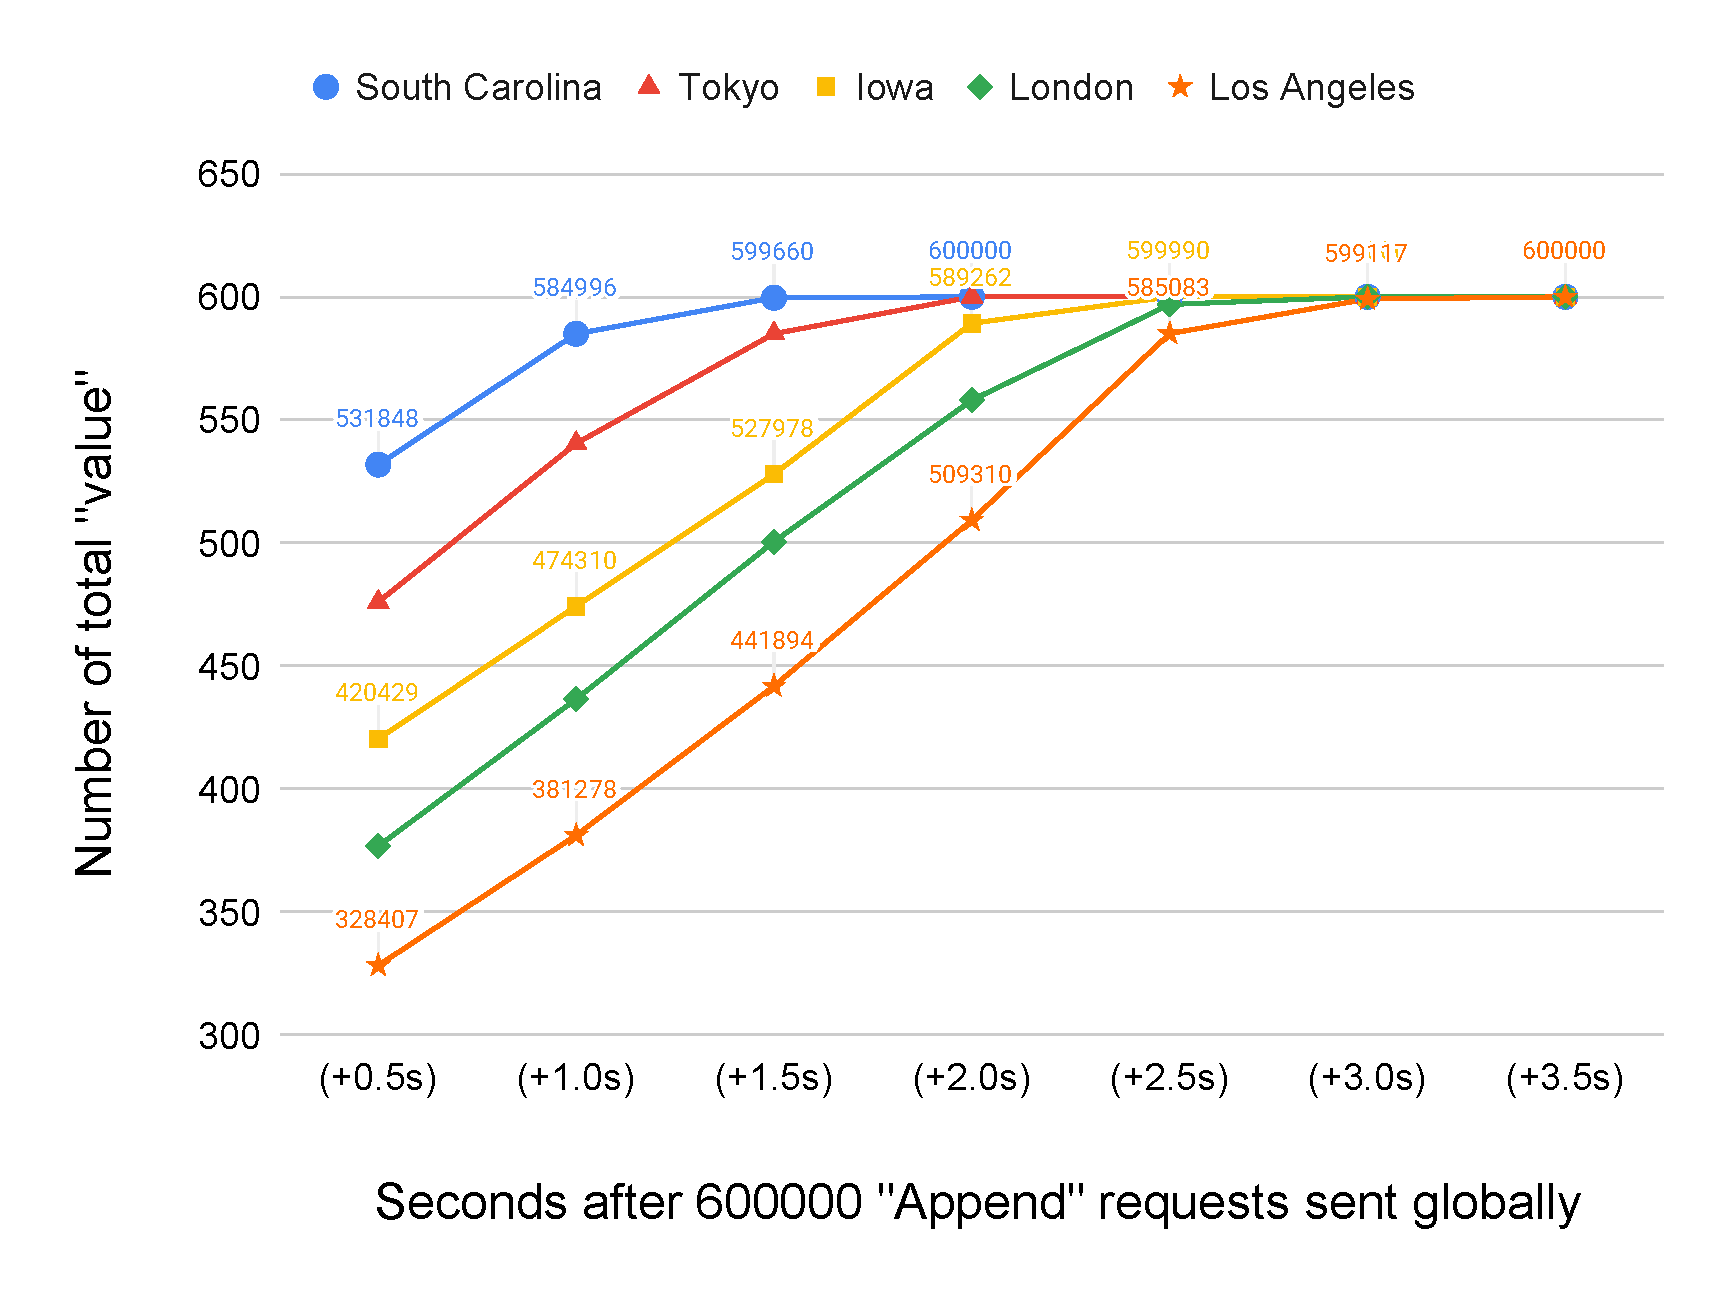
\includegraphics[width=8cm]{figure/consistency.pdf}}
	\subfigure[Get Request Latency.]{\label{fig:g}
		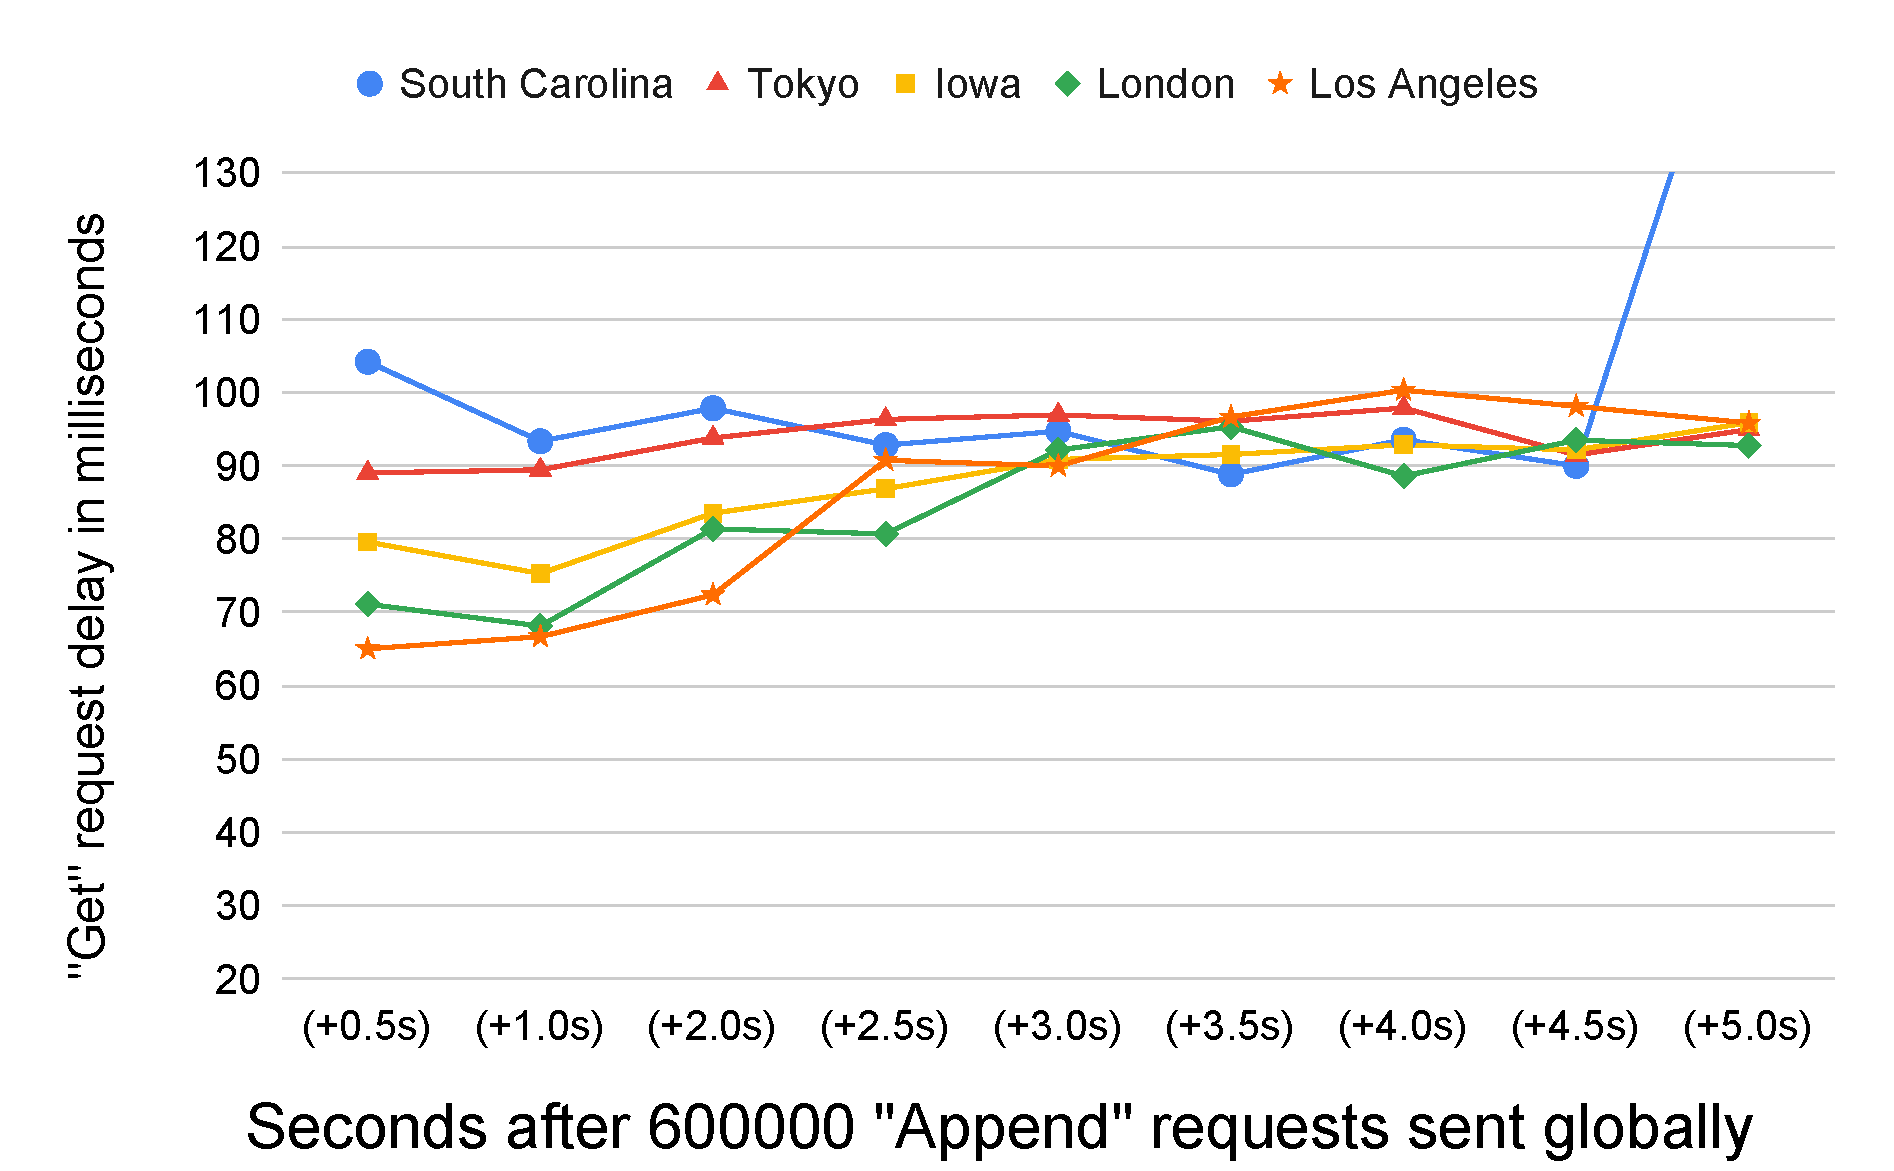
\includegraphics[width=8cm]{figure/GetRequestLatency.pdf}}
\caption{Performance Test Result}
\vspace{-0.4cm}
\label{ConsistencyDelay}
\end{figure}

\subsection{Get Request Performace}
The result of the \texttt{Get} is shown in Figure \ref{GetRequestLatency}. From the figure, we can see the latency starts differently because the Follower held different amount of data. After 3.5 seconds, the latency of different Followers converged to between 90 milliseconds and 100 milliseconds. Note that the implementation of the \texttt{Get} could be optimized to achieve even better performance.

% Get request delay figure
%\begin{figure}[h]
%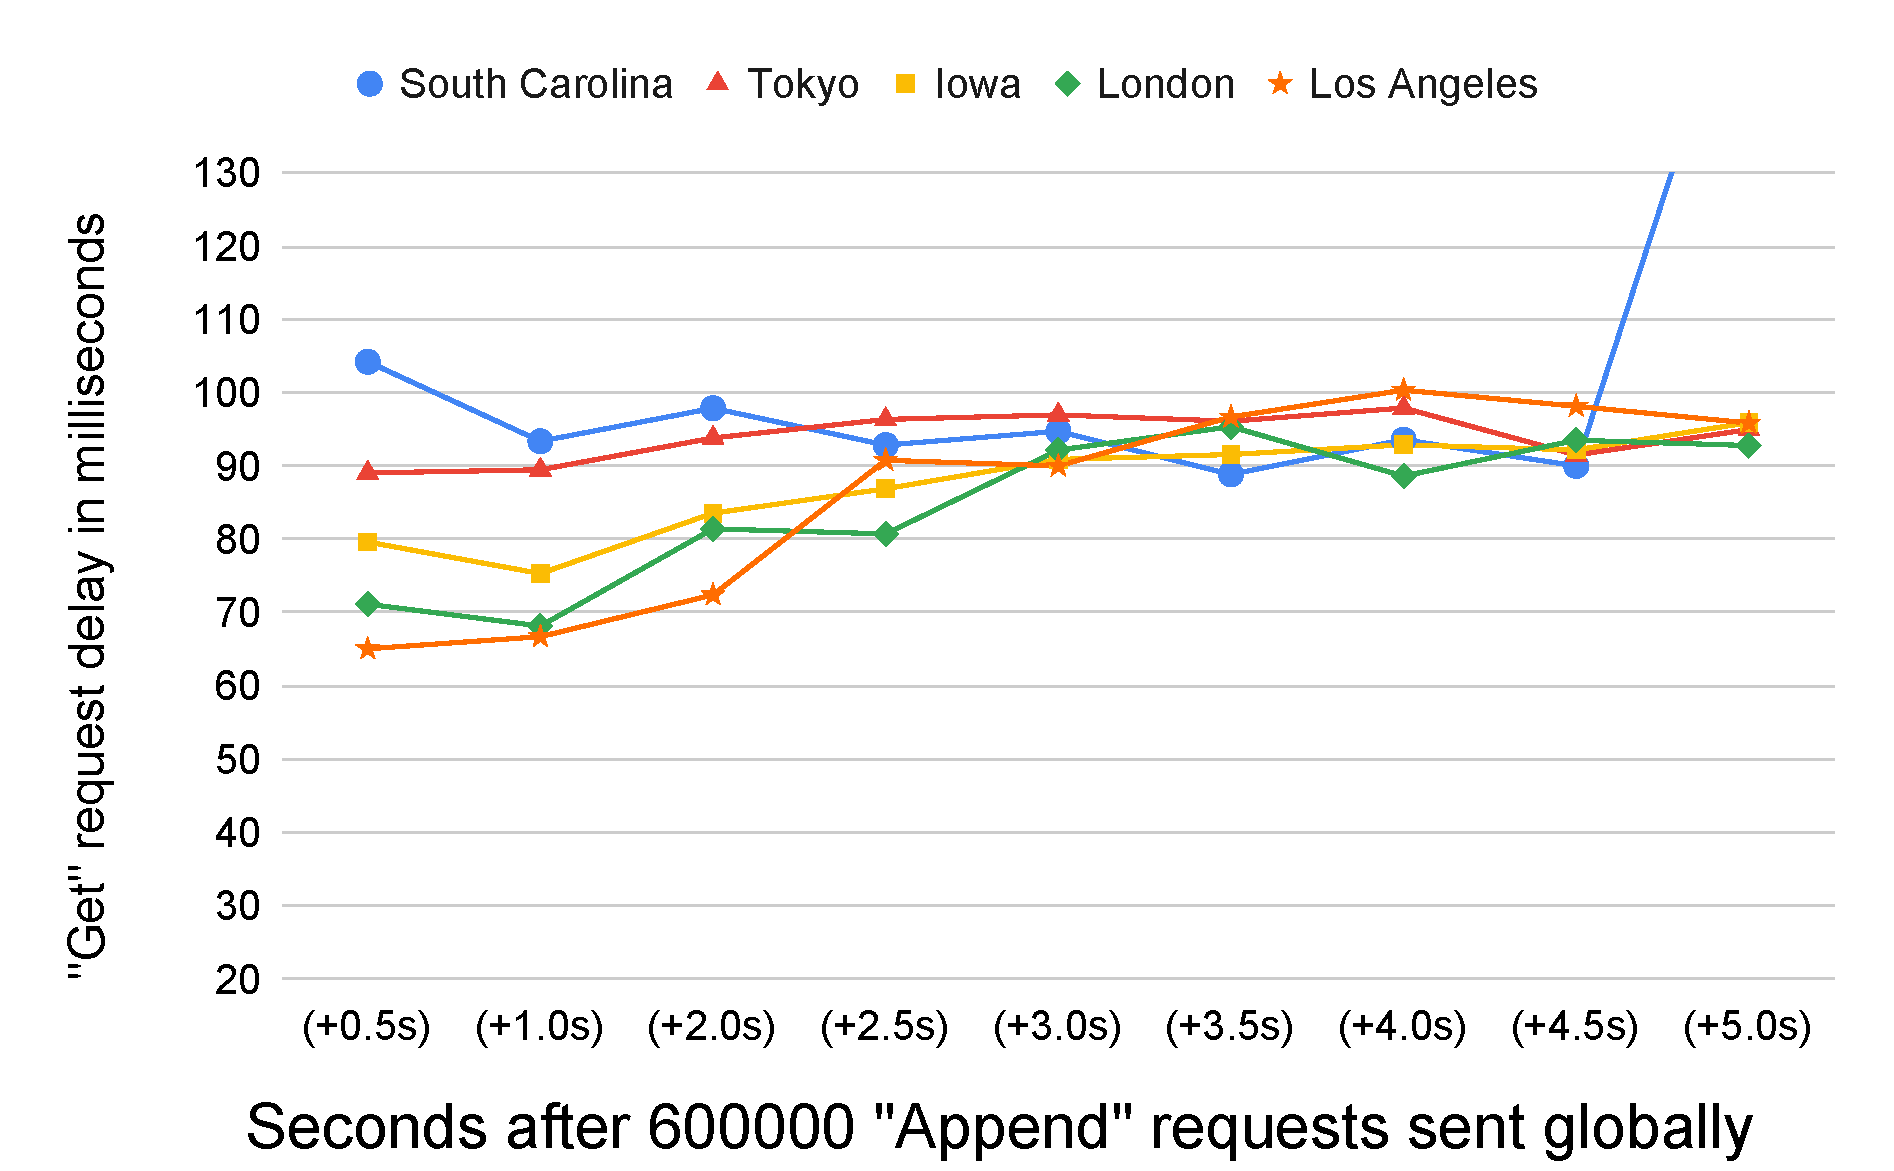
\includegraphics[width=8cm]{figure/GetRequestLatency.pdf}
%\caption{Get Request Latency}
%\label{GetRequestLatency}
%\end{figure}
\vspace{-0.4cm}
\section{Future Work}
We could greatly increase throughput by providing a client library (rather than
a raw GRPC interface) that is aware of the indices or latest index it holds.
This would enable followers to selectively return only the few missing pieces of
data a client is missing rather than all the data.

To increase fault tolerance, we have discussed making each follower and the
leader their own small cluster of consensus nodes. This would greatly increase
fault tolerance and, while it may complicate the system, would not complicate
clients or the protocols via which nodes communicate.

Lastly, there may be cases where followers fail or are partitioned from their
nearby clients. In these cases, we would like to explore whether clients can
fall back to another follower.
\vspace{-0.3cm}
\section{Conclusions}
We built a datastore to provide low latency and high availability for append-only
data storage. While this work is tailed to a specific set of workloads, there
are numerous applications that can benefit from this approach.

Our system can be used to support distributed services such as distributed
monitoring and chat applications with high performance. Importantly, it exposes
a simple interface allowing for simple clients. We believe that this makes it a
useful tool in building distributed and microservice systems.
\vspace{-0.4cm}
\bibliography{paper} 
\bibliographystyle{ieeetr}

\end{document}
